% Options here are passed to the article class.
% Most common options: 10pt, 11pt, 12pt
\documentclass[10pt]{datasheet}

% Input encoding and typographical rules for English language
\usepackage[utf8]{inputenc}
\usepackage[english]{babel}
\usepackage[english]{isodate}

% tikz is used to draw images in this example, but you can
% also use \includegraphics{}.
\usepackage{graphicx}

% These define global texts that are used in headers and titles.
\title{IM02: 1000 Item RAM}
\author{Andrews54757}
\tags{item-memory, random-access}
\date{December 2022}
\revision{Revision 1}

\begin{document}
\maketitle

\section{Features}

\begin{itemize}
\item{Has 1000 different codes/item types. a dropper of storage per code.}
\item{Random access. Can insert and retrieve items in constant time in any order.}
\item{Half hopperspeed order throughput. Can execute insertions and retrievals every 16 game ticks (exclusive, can't do both at same time).}
\item{Hopperlocked. Is fully hopperlocked.}
\item{Togglestateless. No piston toggle states.}
\end{itemize}

\section{Applications}
\begin{itemize}
\item{Temp storage for merging.}
\item{Dynamic bulk mapping storage.}
\end{itemize}

\section{General Description}
The IM02 is able to store and retrieve items with a specific decimal code. This may be useful as a temp storage in an encoded dynamic sorting system.
\vfill\break

\begin{figure}[h]
    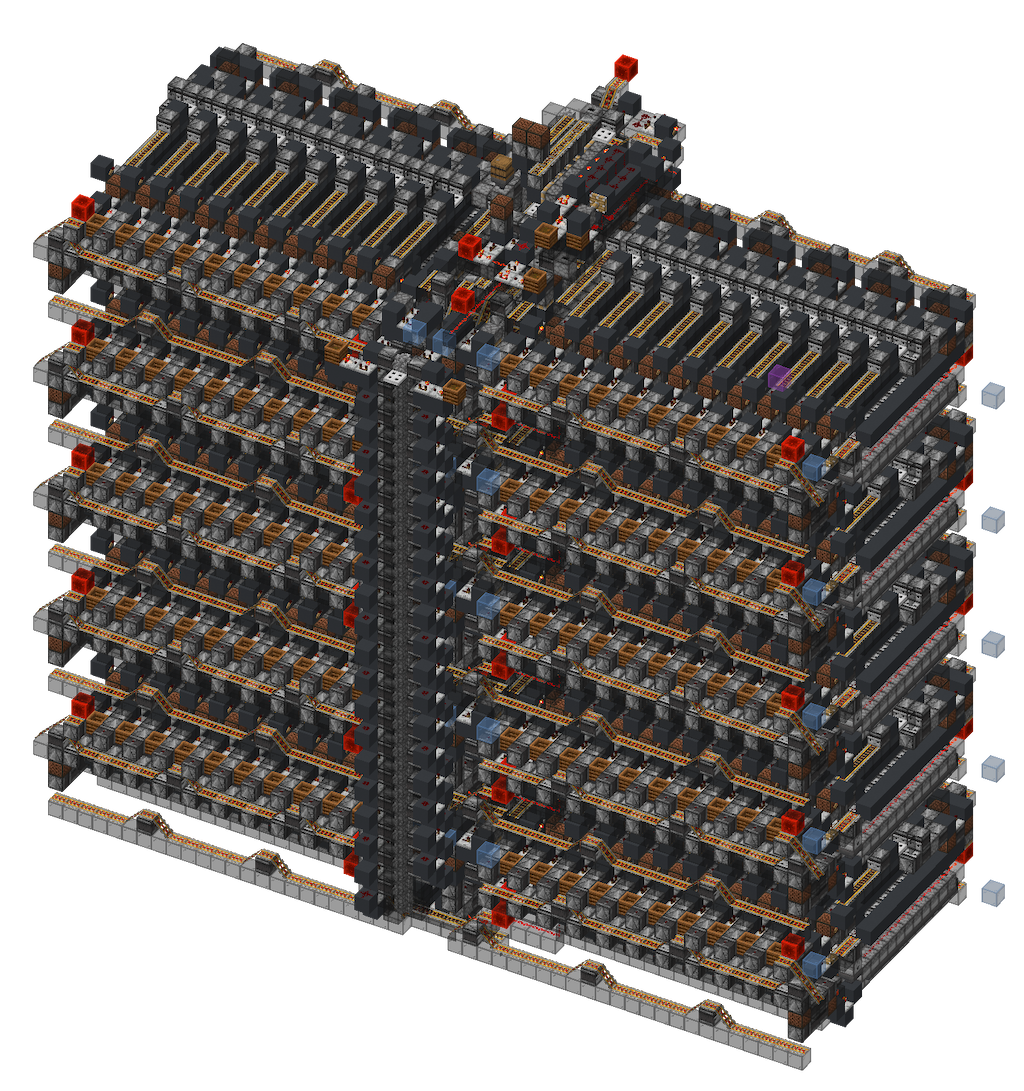
\includegraphics[width=0.45\textwidth]{ram2.png}
    \caption{1000 Item RAM}
\end{figure}

% For wide tables, a single column layout is better. It can be switched
% page-by-page.
\onecolumn
\section{Device Specifications}

\begin{table}[h]
    \caption{Inputs}
    \begin{tabularx}{\textwidth}{l | c | X}
        \thickhline
        \textbf{Name} & \textbf{Range} & \textbf{Description} \\
        \hline
        Code Digit 1 & 1-10 & First digit indicating leaf. \\
        Code Digit 2 & 1-10 & Second digit indicating row. \\
        Code Digit 3 & 1-10 & Third digit indicating column. \\
        \hline
        Execute insertion & Pulse & Executes insertion with the given settings. \\
        \hline
        Execute retrieval & Pulse & Executes retrieval with the given settings. \\
        \hline
        Item Input & Item & Item to be inserted/retrieved. \\
        \thickhline
\end{tabularx}
\end{table}

\begin{table}[h]
    \caption{Outputs}
    \begin{tabularx}{\textwidth}{l | c | X}
        \thickhline
        \textbf{Name} & \textbf{Range} & \textbf{Description} \\
        \hline
        Item Output & Item & Output for retrieval orders. \\
        \thickhline
\end{tabularx}
\end{table}

\begin{table}[h]
    \caption{Device Specifications}
    \begin{tabularx}{\textwidth}{l | c c c | c | X}
        \thickhline
        \textbf{Parameter} & \textbf{Min.} & \textbf{Typ.} & \textbf{Max.} &
        \textbf{Unit} & \textbf{Conditions} \\
        \hline
        Order Execution Interval & 16 & - & - & gt & Normal Usage\\
        \hline
        Hopper Count & & 1111 & & Hoppers & \\
        \hline
        MC Version & 1.13 & 1.17.1 & - & MCV & Latest version at time of writing: 1.19.3\\
        \hline
        Dimensions & & 53 x 55 x 28 & & Blocks & \\
        \thickhline
\end{tabularx}
\end{table}
\newpage

\section{Testing Data}

\begin{table}[h]
\caption{Executed Tests}
\begin{tabularx}{\textwidth}{l | X}
    \thickhline
    \textbf{Test} & \textbf{Result} \\
    \hline
    Insertion & Items were successfully inserted in all positions. \\
    \hline
    Retrieval & Items were successfully retrieved from all positions. \\
    \thickhline
\end{tabularx}
\end{table}

\section{Download Information}
\begin{table}[h]
    \caption{Download Information}
    \begin{tabularx}{\textwidth}{l | l | l | X}
        \thickhline
        \textbf{Identifier} & \textbf{MC} & \textbf{File} & \textbf{Description} \\
        \hline
        IM02 & 1.17.1 & \href{https://github.com/Soontech-Annals/Archive/blob/8413f90a054b6c415703bae02badeba7541344f6/Archive/item-memory/IM02\%201000\%20Item\%20RAM/IM02\_1000\_item\_RAM\_p2.litematic?raw=1}{IM02\_1000\_item\_RAM\_p2.litematic} & Litematic of item RAM device. \\
        \thickhline
    \end{tabularx}
\end{table}

\end{document}